\documentclass[11pt]{article}
\usepackage[utf8]{inputenc}
\usepackage{amsmath}
\usepackage{amsfonts}
\usepackage{amssymb}
\usepackage{graphicx}
\usepackage[super]{nth}
\usepackage{amsthm}
\usepackage{bm}
\newtheorem{theorem}{Theorem}
\newtheorem{objective}{Objective}
\newtheorem{model}{Model}
\usepackage{xcolor}
\definecolor{light-gray}{gray}{0.95}
\newcommand{\code}[1]{\colorbox{light-gray}{\texttt{#1}}}
\usepackage{listings}
\usepackage{placeins}
\usepackage{enumitem}
\usepackage[T1]{fontenc}

\usepackage[authoryear]{natbib}

\lstset{language=R}


\makeatletter
\renewcommand{\maketitle}{
\begin{center}

\pagestyle{empty}

{\Large \bf \@title\par}
\vspace{1cm}

{\LARGE Marcel Gietzmann-Sanders}\\[1cm]

STAT651 - Statistical Theory I \\
University of Alaska Fairbanks


\end{center}
}\makeatother


\title{Homework 9}

\date{2025}
\setcounter{tocdepth}{2}
\begin{document}
\maketitle


\section*{Question 1}

\subsection*{a)}

$$f_Y(y) = \int_0^y 2e^{-(x+y)}dx=-2e^{-(x+y)}\Big|_0^y=2e^{-y}-2e^{-2y}$$

As $e^{-y}>e^{-2y}$ this is a positive function. 

$$\int_0^{\infty}\left( 2e^{-y}-2e^{-2y} \right)dy =2\left( -e^{-y}+e^{-2y}/2 \right)\Big|_0^{\infty}$$

$$=2\left(1 - 1/2 \right)=1$$

So this is in fact a pdf. 

\subsection*{b)}

$$f_{X|Y}(x|y)=\frac{f(x,y)}{f(y)}=\frac{2e^{-(x+y)}}{2e^{-y}-2e^{-2y}}=\frac{e^{-x}}{1-e^{-y}}I(0<x<y<\infty)$$

Given $y>0$ this will always be positive. 

$$\int_0^{y} \frac{e^{-x}}{1-e^{-y}} dx = \frac{1}{1-e^{-y}} \left(-e^{-x} \right)\Big|_0^y=\frac{-e^{-y}+1}{1-e^{-y}}=1$$

So this is indeed a pdf. 

\subsection*{c)}

First we need to find $f_X(x)$:

$$f_X(x)=\int_x^{\infty}2e^{-(x+y)}dy=-2e^{-(x+y)}\Big|_x^{\infty}=2e^{-2x}$$

Then:

$$f_{X|Y}(x|y)=\frac{f(x,y)}{f(x)}=\frac{2e^{-(x+y)}}{2e^{-2x}}I(0<x<y<\infty)=\frac{e^{-y}}{e^{-x}}I(0<x<y<\infty)$$

Both the numerator and denominator are positive so this quantity is also positive. 

$$\int_x^{\infty}\frac{e^{-y}}{e^{-x}}dy=\frac{1}{e^{-x}}\left( -e^{-y}\right)\Big|_x^{\infty}=\frac{0+e^{-x}}{e^{-x}}=1$$

So this is indeed a pdf. 

\subsection*{d)}

$X$ and $Y$ are not independent as you cannot factor $I(0<x<y<\infty)$ into components only of $x$ and $y$. 

\section*{Question 2}

\subsection*{a)}

\begin{figure}[h!] 
	\centering
  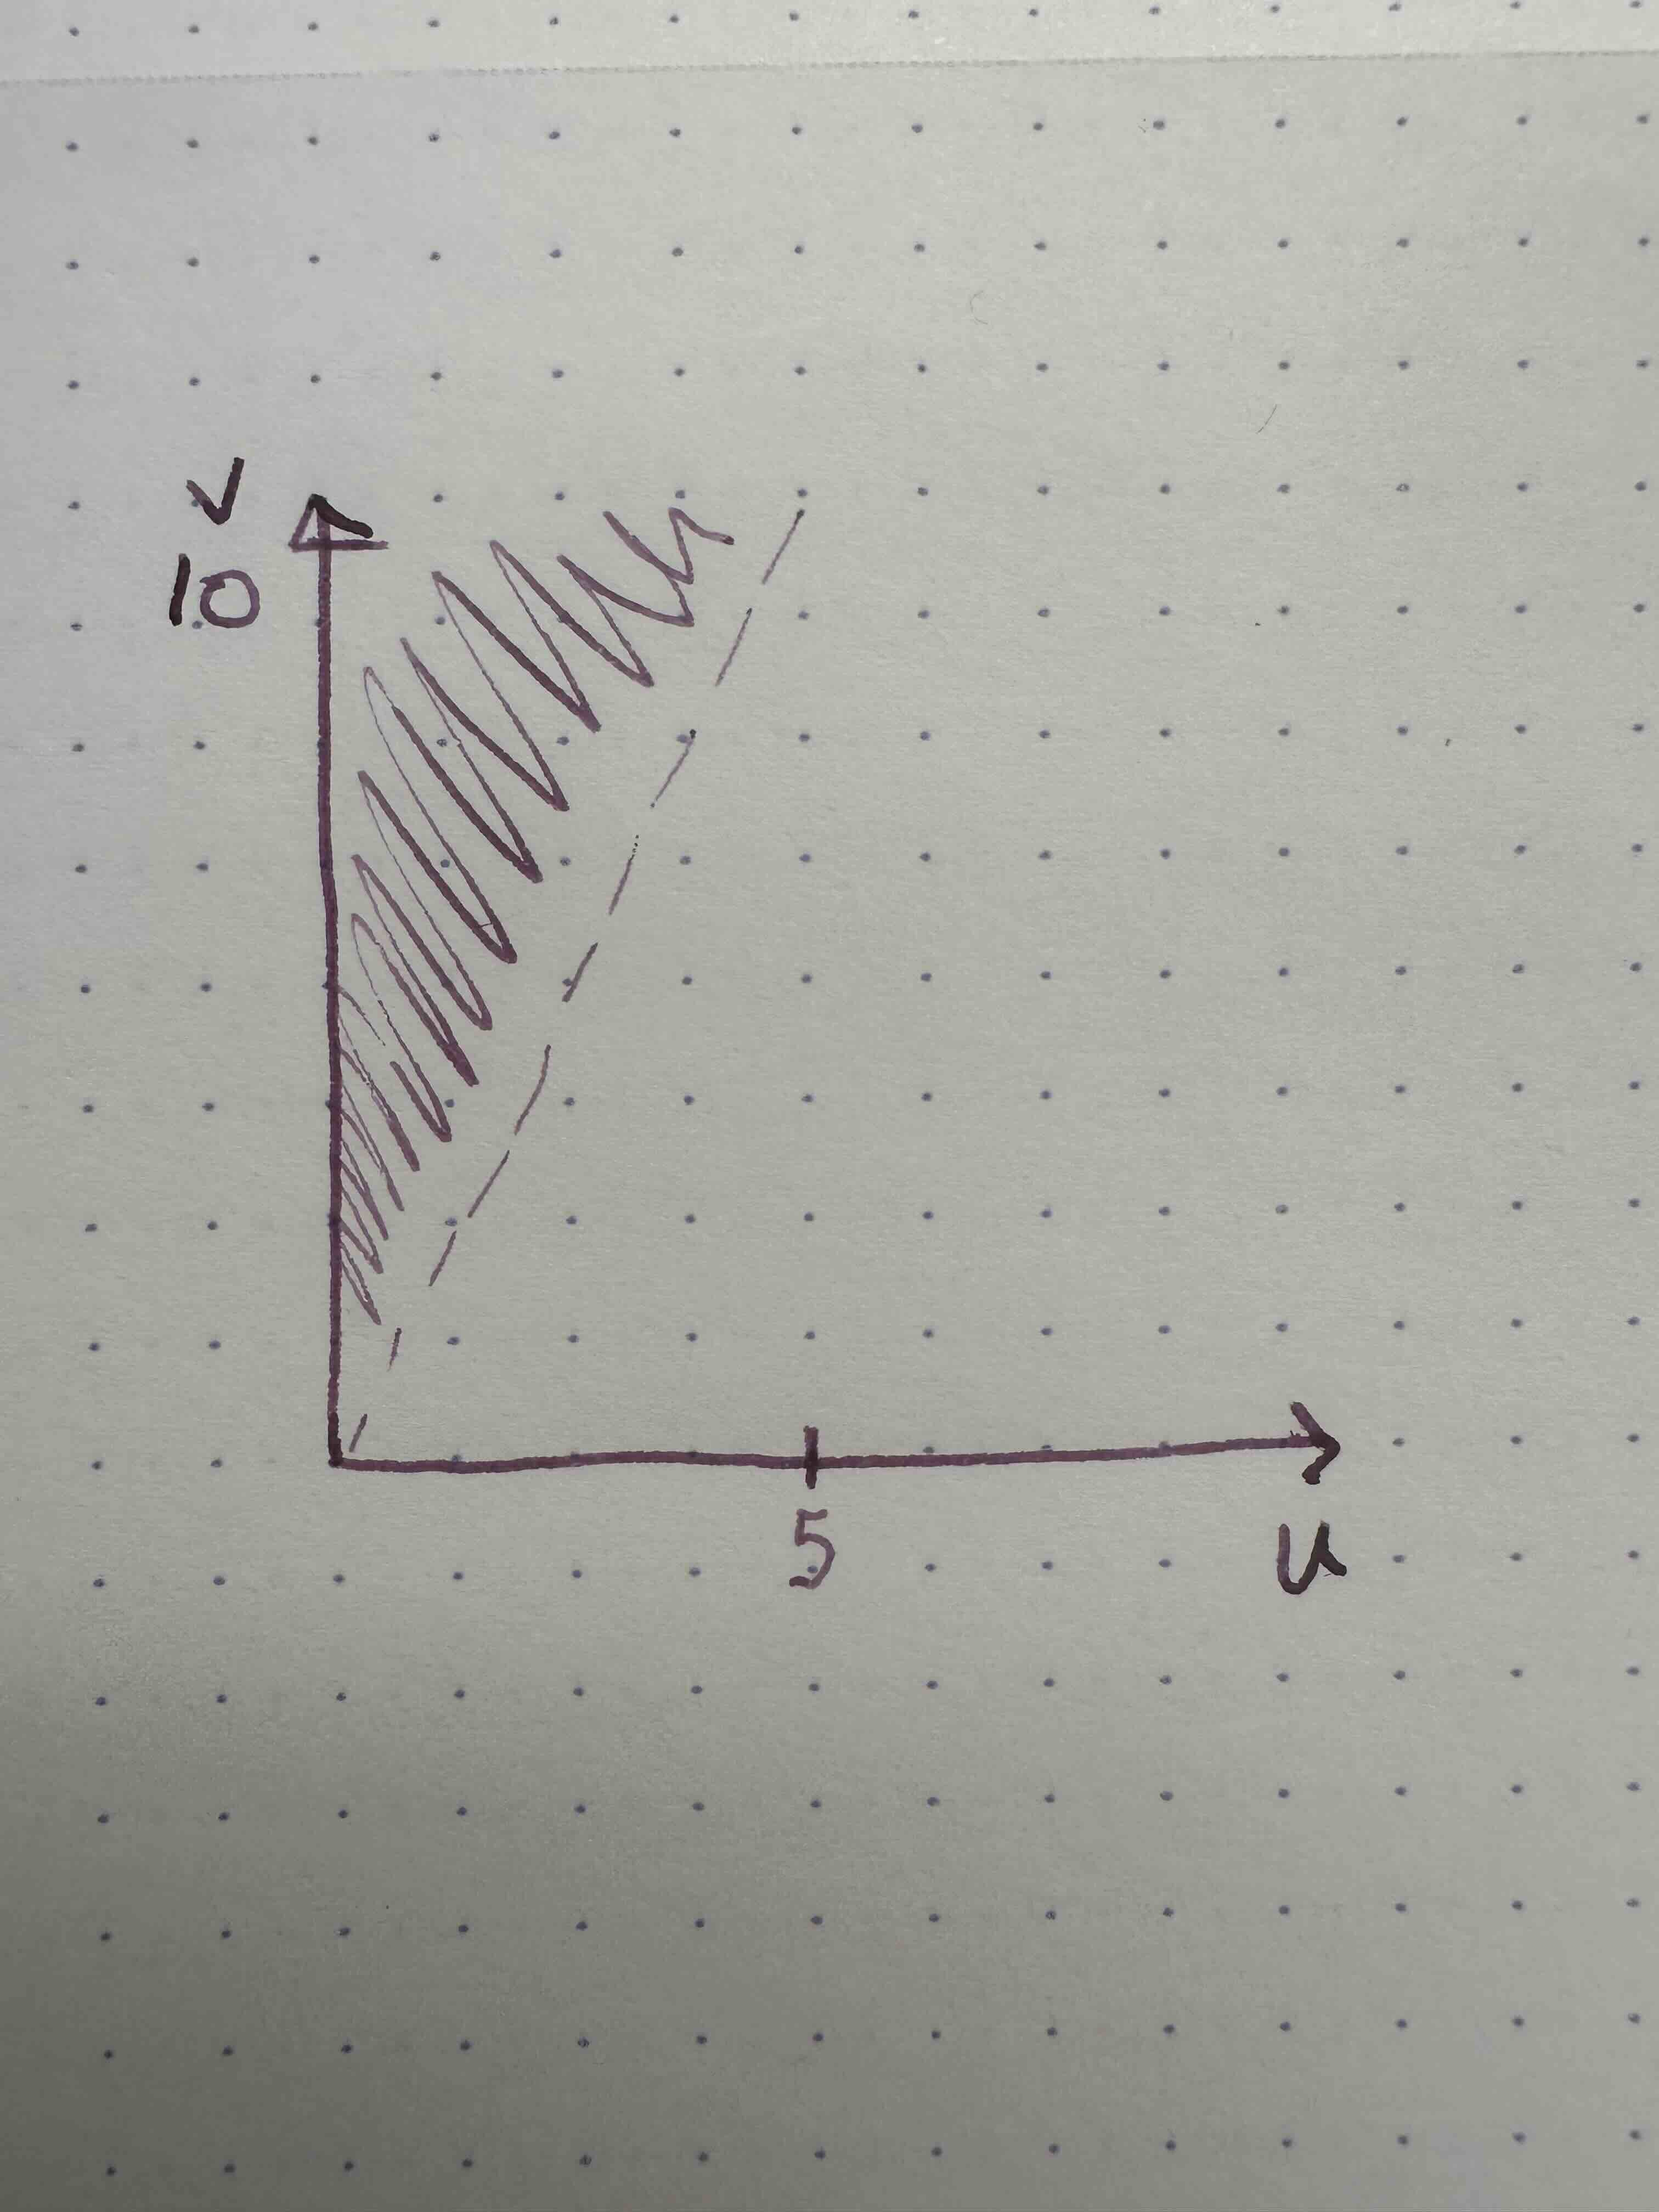
\includegraphics[height=40mm]{HW9F1.jpg}
  \label{fig:tree}
\end{figure}

\FloatBarrier

\subsection*{b)}

We have: $x=u$ and $y=v-u$. So: 

$$
\det{\begin{bmatrix}
    \frac{\partial x}{\partial u} & \frac{\partial x}{\partial v} \\
    \frac{\partial y}{\partial u} & \frac{\partial y}{\partial v}
\end{bmatrix}}
=
\det{\begin{bmatrix}
    1 & 0 \\
    -1 & 1
\end{bmatrix}}
= 1 - 0 = 1
$$

Therefore: 

$$f_{U,V}(u,v) = 2e^{-v}I(0<u<\infty)I(2u<v<\infty)$$

\subsection*{c)}

$$f_U(u) = \int_{2u}^{\infty}2e^{-v}dv=2\left( -e^{-v} \right)\Big|_0^{\infty}= 2e^{-2u}$$

$$f_V(v) = \int_0^{v/2}2e^{-v}du=2e^{-v}\left(u \right)\Big|_0^{v/2}=ve^{-v}$$

\subsection*{d)}

Once again $U$ and $V$ are not independent because we cannot factor the $I$ in terms of functions only of $v$ and $u$. 

\section*{Question 3}

$f_X(x) = ce^{-x^2/a}$, $f_Y(y) = ce^{-y^2/a}$ and therefore as $X$ and $Y$ are independent: $$f_{X,Y}(x,y)=c^2e^{-(x^2+y^2)/a}$$

Now $y=v$ and $x=uv$ so that:

$$
\det{\begin{bmatrix}
    \frac{\partial x}{\partial u} & \frac{\partial x}{\partial v} \\
    \frac{\partial y}{\partial u} & \frac{\partial y}{\partial v}
\end{bmatrix}}
=
\det{\begin{bmatrix}
    v & u \\
    0 & 1
\end{bmatrix}}
= v
$$

which in turn means that:

$$f_{U,V} = c^2e^{-(u^2v^2+v^2)/a}|v|=c^2e^{-v^2(u^2+1)/a}|v|$$

As this function is symmetric in $v$ around $0$ we have: 

$$f_U(u) = 2\int_0^{\infty}c^2e^{-v^2(u^2+1)/a}vdv $$

$$=\frac{-c^2ae^{-v^2(u^2+1)/a}}{(u^2+1)}\Big|_0^{\infty}=\frac{c^2a}{(u^2+1)}$$

As $c=\sqrt{2\pi}$ and $a=2$ this becomes:

$$f_U(u) = \frac{1}{\pi(u^2+1)}$$

which is the pdf for the Cauchy distribution.

\section*{Question 4}

Let $V=X$. Then we have $x = v$ and $y= u-v$. This means that:

$$
\det{\begin{bmatrix}
    \frac{\partial x}{\partial u} & \frac{\partial x}{\partial v} \\
    \frac{\partial y}{\partial u} & \frac{\partial y}{\partial v}
\end{bmatrix}}
=
\det{\begin{bmatrix}
    0 & 1 \\
    1 & -1
\end{bmatrix}}
= 0 - (1) = -1
$$

This means that our $f(x,y)$ gets multiplied by $1$ in the conversion to $f(u,v)$. Because our $f(x,y)=2$ in all cases this means $f(u,v)=2$ in all cases as well. To get $f_U(u)$ we therefore now just need to find the marginal distribution of $U$ which will be all about understanding the bounds of integration. 

\subsection*{a)}

In this case, for a given $u$, $v$ can range from $0$ to $u$. 

$$f_U(u) = \int_0^{u}2dv = 2u$$

where $u$ can range from $0\rightarrow 1$. That is $f_U(u) = 2uI(0 \leq u \leq 1)$.

\subsection*{b)}

In this case, for a given $u$, $v$ can range from $0$ to $u/2$ (as $x\leq y$). 

$$f_U(u) = \int_0^{u/2}2dv = u$$

In this case $u$ can range from $0$ to $2$ so $f_U(u) = uI(0\leq u \leq 2)$.

\subsection*{c)}

In this case, if $u>1$ then $v$ can range from $u-1 \rightarrow 1$. If $u<1$ then $v$ ranges from $0 \rightarrow u$. 

That is:

$$
f_U(u) =
   \begin{cases} 
      \int_0^u dv = u & 0\leq u \leq 1 \\
      \int_{u-1}^1 dv = 2 - u & 1 < u \leq 2
   \end{cases}
$$

\section*{Question 5}

\subsection*{a)}

$$M_{X+Y}(t) = M_X(t) M_Y(t) = \left( \frac{1}{1-\beta t}\right)^{\alpha_x} \left( \frac{1}{1-\beta t}\right)^{\alpha_y}=\left( \frac{1}{1-\beta t}\right)^{\alpha_x+\alpha_y}$$

So $X+Y \sim \text{Gamma}(\alpha_x + \alpha_y, \beta)$

\subsection*{b)}

$$M_{X+Y}(t) = M_X(t) M_Y(t) = e^{\theta (e^t -1)} e^{\lambda (e^t -1)} = e^{(\theta + \lambda) (e^t -1)}  $$

So $X+Y \sim \text{Poisson}(\theta + \lambda)$

\section*{Question 6}

In this case we have a hierarchical model $Z|N$. 

$$\mathbb{E}(Z)=\mathbb{E}(\mathbb{E}(Z|N))$$

$$\mathbb{E}(Z|N) = \mathbb{E}\left(\sum_{i=1}^N Y_i\right) = \sum_{i=1}^N\mathbb{E}(Y_i)=10N$$


$$\mathbb{E}(Z) = \mathbb{E}(\mathbb{E}(Z|N)) = \sum_{N=1}^{13} \frac{1}{13} 10N=70$$

Now onto the variance.

$$\text{Var}(Z) = \text{Var}(\mathbb{E}(Z|N)) + \mathbb{E}(\text{Var}(Z|N))$$

Let's start with the first of those two terms:

$$\text{Var}(\mathbb{E}(Z|N)) = \mathbb{E}(\mathbb{E}(Z|N)^2)-\mathbb{E}(\mathbb{E}(Z|N))^2$$
$$=\sum_{N=1}^{13} \frac{1}{13} (10N)^2 - 70^2=6300-4900=1400$$

And then the second of the two terms:

$$\text{Var}(Z|N)=\text{Var}\left( \sum_{i=1}^{N} Y_i \right)=\sum_{i=1}^{N} \text{Var}\left( Y_i \right)=10N$$

$$\mathbb{E}(\text{Var}(Z|N)) = \sum_{N=1}^{13}\frac{1}{13}10N=70$$

Therefore:

$$\text{Var}(Z) = \text{Var}(\mathbb{E}(Z|N)) + \mathbb{E}(\text{Var}(Z|N))=1400 + 70= 1470$$


\section*{Question 7}

$$P(Y<y)=P(WX < y)$$ 
By independence of $W$ and $X$ we have:

$$P(WX < y)=P(X < y)P(W=1) + P(X > -y)P(W=-1)$$

Given $N(0,1)$ is symmetric around $0$, $P(X>-y) = P(X<y)$. Therefore we have:

$$P(Y<y)=P(X<y)\left(P(W=1) + P(W=-1)\right)=P(X<y)$$

As $X$ and $Y$ share the same cdf and support they must also share the same pdf. 

\section*{Question 8}

\subsection*{a)}

Let $\mu_Y = \mathbb{E}(Y)$, $\mu_{X_1} = \mathbb{E}(X_1)$, and $\mu_{X_2}=\mathbb{E}(X_2)$ then:

$$\text{cov}(X_1 + X_2, Y) = \mathbb{E}\left((X_1 + X_2 - \mu_{X_1} - \mu_{X_2})(Y - \mu_Y)\right)$$

by virtue of the fact that $\mathbb{E}(X_1 + X_2) = \mu_{X_1} + \mu_{X_2}$ 

$$(X_1 + X_2 - \mu_{X_1} - \mu_{X_2})(Y - \mu_Y) = X_1Y -X_1\mu_Y + X_2Y - X_2\mu_Y $$
$$- ( \mu_{X_1}Y -\mu_{X_1}\mu_Y + \mu_{X_2}Y - \mu_{X_2}\mu_Y)=(X_1Y -X_1\mu_Y - (\mu_{X_1}Y -\mu_{X_1}\mu_Y)) $$
$$+(X_2Y - X_2\mu_Y- (\mu_{X_2}Y - \mu_{X_2}\mu_Y))=(X_1-\mu_{X_1})(Y- \mu_Y)$$
$$+(X_2-\mu_{X_2})(Y- \mu_Y)$$

Therefore:

$$\text{cov}(X_1 + X_2, Y) = \mathbb{E}\left((X_1 + X_2 - \mu_{X_1} - \mu_{X_2})(Y - \mu_Y)\right)$$
$$=\mathbb{E}\left((X_1-\mu_{X_1})(Y- \mu_Y)+(X_2-\mu_{X_2})(Y- \mu_Y)\right)$$
$$=\mathbb{E}((X_1-\mu_{X_1})(Y- \mu_Y)) + \mathbb{E}((X_2-\mu_{X_2})(Y- \mu_Y))$$
$$=\text{cov}(X_1, Y) + \text{cov}(X_2, Y)$$

\subsection*{b)}

$$\text{cov}(X, a) = \mathbb{E}((X-\mathbb{E}(X))(a-\mathbb{E}(a)))$$
$$=\mathbb{E}((X-\mathbb{E}(X))(a-a)))= \mathbb{E}(0)=0$$




\end{document}